% Paquets généraux
\documentclass[a4paper,12pt,titlepage,twoside]{article}
\usepackage[T1]{fontenc}
\usepackage[utf8]{inputenc}
\usepackage[french]{babel}
\usepackage{subcaption}
\addto\captionsfrench{%
  \renewcommand{\tablename}{Tableau}%
}
\usepackage[gen]{eurosym}
%\usepackage[dvips]{graphicx}
\usepackage{minted}
\usepackage{fancyhdr}
\usepackage{pdfpages} 
\usepackage{multido}
\usepackage{hyperref}
\usepackage{textcomp}
\usepackage{schemabloc}
%\usepackage[bitstream-charter]{mathdesign}
\usepackage{array}
\newcolumntype{P}[1]{>{\centering\arraybackslash}p{#1}}
\usepackage[shortlabels]{enumitem}
\usepackage[framemethod=TikZ]{mdframed}

\newcommand{\id}{71}
\newcommand{\nom}{Théorie des mécanismes}
\newcommand{\sequence}{04}
\newcommand{\nomsequence}{Liaisons entre les solides}
\newcommand{\num}{02}
\newcommand{\type}{KH}
\newcommand{\descrip}{Liaisons équivalentes, hyperstatisme, liaisons en série et en parallèle, théorie des graphes}
\newcommand{\competences}{B2-12: Proposer une modélisation des liaisons avec leurs caractéristiques géométriques. \\ &  B2-13: Proposer un modèle cinématique paramétré à partir d'un système réel, d'une maquette numérique ou d'u \\ &  B2-17: Simplifier un modèle de mécanisme. \\ &  B2-18: Modifier un modèle pour le rendre isostatique. \\ &  C1-04: Proposer une démarche permettant d'obtenir une loi entrée-sortie géométrique.  \\ &  C2-05: Caractériser le mouvement d'un repère par rapport à un autre repère. \\ &  C2-06: Déterminer les relations entre les grandeurs géométriques ou cinématiques. }
\newcommand{\nbcomp}{7}
\newcommand{\systemes}{}
\newcommand{\systemesnum}{}
\newcommand{\systemessansaccent}{}
\newcommand{\ilot}{2}
\newcommand{\ilotstr}{02}
\newcommand{\dossierilot}{\detokenize{Ilot_02 }}

%\usepackage{style}
\usepackage{bodegraph}
\usepackage{rpcinematik}
\usepackage[locale = FR]{siunitx}
\usepackage{caption}
\newcommand{\institute}{Lycée Dorian}

\usepackage{listings}
\usepackage{fancyvrb}
\usepackage{color}
\usepackage{xcolor}
\usepackage{colortbl}
\usepackage{helvet}
\usepackage[frenchmath]{newtxsf} % for sans serif symbols
\renewcommand{\familydefault}{\sfdefault}
%\usepackage{amsfonts}
%\usepackage{amsmath}
%\usepackage{lmodern}
\usepackage{mathastext}
%\usepackage{xspace}
\usepackage{varioref}
\usepackage{tabularx}
%\usepackage{floatflt}
\usepackage{graphics}
\usepackage{wrapfig}
\usepackage{textcomp}
\usepackage{tikz,tkz-tab}
\usepackage[european resistor, european voltage, european current]{circuitikz}
\usepackage{wrapfig}
\usepackage{gensymb}
\usepackage[percent]{overpic}
\usetikzlibrary{babel}
\usepackage{ifthen}
\usepackage{cancel}
\usepackage{etoolbox}
\usepackage{multirow}
%\usepackage{boxedminipage}
\definecolor{gris25}{gray}{0.75}
\definecolor{bleu}{RGB}{18,33,98}
\definecolor{bleuf}{RGB}{42,94,171}
\definecolor{bleuc}{RGB}{231,239,247}
\definecolor{bleum}{RGB}{160,195,226}
\definecolor{rougef}{RGB}{185,18,27}
\definecolor{rougec}{RGB}{255,188,204}%255,230,231
\definecolor{vertf}{RGB}{103,126,82}
\definecolor{vertc}{RGB}{220,255,191}
\definecolor{forestgreen}{rgb}{0.13,0.54,0.13}
\definecolor{blcr}{rgb}{0.59,0.69,0.84}
\definecolor{blfr}{rgb}{0.32,0.51,0.75}
\definecolor{orfr}{rgb}{0.90,0.42,0.15}
\definecolor{orcr}{rgb}{0.90,0.65,0.50}
\definecolor{orangef}{rgb}{0.659,0.269,0.072}
\definecolor{orange}{rgb}{0.58,0.35,0.063}
\definecolor{orangec}{rgb}{0.43,0.32,0.25}
\definecolor{rcorrect}{rgb}{0.6,0,0}
\definecolor{sequence}{rgb}{0.75,0.75,0.75}
\definecolor{competences}{rgb}{0.61,0.73,0.35}
\definecolor{rose}{HTML}{ff00ff}
\definecolor{grisf}{HTML}{222222}
\definecolor{grisc}{HTML}{636363}
\definecolor{normal}{HTML}{4087c4}
\definecolor{info}{HTML}{5bc0de}
\definecolor{success}{RGB}{92,184,92}
\definecolor{warning}{RGB}{240,173,78}
\definecolor{danger}{RGB}{217,83,79}
\hypersetup{                    % parametrage des hyperliens
    colorlinks=true,                % colorise les liens
    breaklinks=true,                % permet les retours à la ligne pour les liens trop longs
    urlcolor= blfr,                 % couleur des hyperliens
    linkcolor= orange,                % couleur des liens internes aux documents (index, figures, tableaux, equations,...)
    citecolor= forestgreen                % couleur des liens vers les references bibliographiques
    }

\newcolumntype{M}[1]{>{\centering\arraybackslash}m{#1}}
\definecolor{codegreen}{rgb}{0,0.6,0}
\definecolor{codegray}{rgb}{0.5,0.5,0.5}
\definecolor{codepurple}{rgb}{0.58,0,0.82}
\definecolor{backcolour}{rgb}{0.95,0.95,0.92}

\lstdefinestyle{mystyle}{
    backgroundcolor=\color{backcolour},   
    commentstyle=\color{codegreen},
    keywordstyle=\color{magenta},
    numberstyle=\tiny\color{codegray},
    stringstyle=\color{codepurple},
    basicstyle=\ttfamily\footnotesize,
    breakatwhitespace=false,         
    breaklines=true,                 
    captionpos=b,                    
    keepspaces=true,                 
    numbers=left,                    
    numbersep=5pt,                  
    showspaces=false,                
    showstringspaces=false,
    showtabs=false,                  
    tabsize=2
}

\lstset{style=mystyle}

% Mise en page
\pagestyle{fancy}

\setlength{\hoffset}{-18pt}
\setlength{\oddsidemargin}{0pt} 	% Marge gauche sur pages impaire2s
\setlength{\evensidemargin}{0pt} 	% Marge gauche sur pages paires
\setlength{\marginparwidth}{00pt} 	% Largeur de note dans la marge
\setlength{\headwidth}{481pt} 	 	% Largeur de la zone de tête (17cm)
\setlength{\textwidth}{481pt} 	 	% Largeu\textbf{r de la zone de texte (17cm)
\setlength{\voffset}{-18pt} 		% Bon pour DOS
\setlength{\marginparsep}{7pt}	 	% Séparation de la marge
\setlength{\topmargin}{-30pt} 		% Pas de marge en haut
\setlength{\headheight}{55pt} 		% Haut de page
\setlength{\headsep}{20pt} 		% Entre le haut de page et le texte
\setlength{\footskip}{30pt} 		% Bas de\textbf{ page + séparation
\setlength{\textheight}{700pt} 		% Hauteur de l'icone zone de texte (25cm)
\setlength\fboxrule{1 pt}
\renewcommand{\baselinestretch}{1}
\setcounter{tocdepth}{1}
\newcommand{\cadre}[2]
{\fbox{
  \begin{minipage}{#1\linewidth}
   \begin{center}
    #2\\
   \end{center}
  \end{minipage}
 }
}

\newcommand{\repon}[1]
{
~\ \\
\begin{tabular}{|m{\linewidth}|}
 \hline
\multido{}{#1}{\\ \hline}
\end{tabular}
}


\newcommand{\objectif}[1]{
\mdfsetup{%
frametitle={%
\tikz[baseline=(current bounding box.east),outer sep=0pt]
\node[anchor=east,rectangle,fill=bleum]
{\strut Objectif~};}}
\mdfsetup{innertopmargin=10pt,linecolor=bleum,%
linewidth=2pt,topline=true,%
frametitleaboveskip=\dimexpr-\ht\strutbox\relax
}
\begin{mdframed}[]\relax%
#1
\end{mdframed}}


\newcounter{num_quest} \setcounter{num_quest}{0}
\newcounter{num_rep} \setcounter{num_rep}{0}
\newcounter{num_cor} \setcounter{num_cor}{0}

\newcommand{\feuilleDR}[1]{
	\begin{tikzpicture}
		\draw[gray!30](0,0)grid[step=0.5cm](\linewidth,#1);
	\end{tikzpicture}
}

%\newcommand{\question}[1]{\refstepcounter{num_quest}\par
%~\ \\ \parbox[t][][t]{0.15\linewidth}{\textbf{Question \arabic{num_quest}}}\parbox[t][][t]{0.85\linewidth}{#1\label{q\the\value{num_quest}}}\par
%}

\newcommand{\question}[1]{\refstepcounter{num_quest}\par
~\ \\ \textbf{Question \arabic{num_quest} : }#1\label{q\the\value{num_quest}}\par
}

\newcommand{\posetafigure}[3]{
\begin{figure}[ht!]
 \begin{center}
  \includegraphics[width=#2\linewidth]{img/#1}
 \end{center}
 \caption{\label{#1} #3}
\end{figure}}

\newcommand{\goforum}{
\begin{figure}

\end{figure}
\begin{center}
 
\includegraphics[width=0.7\linewidth]{../../../img/go_forum}
\end{center}
\label{go_forum}
\caption{J'pète les plombs}
\end{figure}}

\newcommand{\reponse}[4][1]
{\noindent
\parbox{\textwidth}{
\rule{\linewidth}{.5pt}\\
\textbf{Question\ifthenelse{#1>1}{s}{} \multido{}{#1}{%
\refstepcounter{num_rep}\ref{q\the\value{num_rep}} }:} ~\ \\
\ifdef{\public}{#3 \ifthenelse{#2>0}{~\ \\ 	\feuilleDR{#2}}}{#4}
}}

\newcommand{\cor}
{\refstepcounter{num_cor}
\noindent
\rule{\linewidth}{.5pt}
\textbf{Question \arabic{num_cor}:} \\
}

\newcommand{\finsujet}
{
    \begin{center}
    \Large{FIN}
    \end{center}

    \cleardoublepage

    \ifdef{\public}{\pagestyle{docreponse}}{\pagestyle{correction}}

    \ifdef{\public}{
        \begin{tikzpicture} 
            \draw (0,0) rectangle (2,2);
            \draw (0,0) -- (2,2);
            \draw (1.5,0.5) node {\large 20};
            \draw (2.5,0) rectangle (16,2);
            \draw (4.5,1.7) node {\large Commentaires:};
        \end{tikzpicture}
    }
    ~\ \\
}


%\newcommand{\repcarre}[2]
%{
%~\ \\
%\begin{tikzpicture}
%\draw [fill=white] (0,0) rectangle +(\linewidth,#1);
%\node[align=left] at (1.1,#2-0.3) {\textbf{Question #1:}};
%\end{tikzpicture}
%}

\newcommand{\titre}[1]
{\begin{center}
\cadre{0.8}{\huge #1} 
\end{center}
}


%Définition des torseurs :
\newcommand{\torseur}[2]{\left\{\mathcal{#1}_{#2} \right\}}
\newcommand{\torseurh}[3]{\left\{\genfrac{}{}{0pt}{0}{#1}{#2}\right\}_{#3}}
\newcommand{\torseurv}[8]{\left\{
\begin{matrix}
#1 & #4 \\ #2 & #5 \\ #3 &#6
\end{matrix}
\right\}_{{#7},{#8}}}

%Définition des torseurs :
%\newcommand{\torseur}[2]{\left \{\mbox{\relsize{2}{$\mathcal {#1}$}\relsize{-2}}\phantom{}_{\mbox{\scriptsize $#2$}} \right \}}
%\newcommand{\torseurh}[3]{\left\{\genfrac{}{}{0pt}{0}{#1}{#2}\right\}_{#3}}
%\newcommand{\torseurv}[8]{
%\left\{\begin{array}{@{}c|c@{}} #1 & #4 \\ #2 & #5 \\ #3 & #6 \end{array} \right\}_{#7,#8}
%}
\newcommand{\derivee}[2]{\left.\dfrac{\d #1}{\d t}\right|_{#2}}
\newcommand{\tripleint}{\int\!\!\!\!\!\int\!\!\!\!\!\int}

% Notation cinématique et statique
\newcommand{\cinematique}[2]{\mbox{#1}/\mbox{#2}}
\newcommand{\statique}[2]{\mbox{#1}\rightarrow\mbox{#2}}
\newcommand{\moment}[3]{\vv {#1}_{\scriptsize{#3}}(#2)}
\newcommand{\resultante}[2]{\vv {#1}_{\scriptsize{#2}}}


%Commande de base
\newcommand{\jo}{\left(j\omega\right)} % j \omega dans l'analyse fréquentielle
\newcommand{\tl}{\xrightarrow{\mathcal{L}}} % transformée de laplace sur fleche
\newcommand{\tli}{\xrightarrow{\mathcal{L}^{-1}}} % transformée inverse de laplace sur fleche
\renewcommand{\d}[1][]{\mathrm{d#1}}
\newcommand{\dd}[1][]{\mathrm{d#1}}
\newcommand{\vect}[2]{{#1}\wedge{#2}}
\newcommand{\base}[3]{(\vec #1,\vec #2,\vec #3)}
\newcommand{\vectbase}[4]{{\vphantom{\left| \begin{matrix}
#1\\#2\\#3 \end{matrix} \right|}}_{#4}{\left| \begin{matrix}
#1\\#2\\#3 \end{matrix} \right.}}
%Pour avoir les paragraphes sous la forme I, II, III
\renewcommand{\thesection}{\Roman{section}}
\setcounter{secnumdepth}{3}
\renewcommand{\Frlabelitemii}{$\bullet$}

% En tête et pied de page
\lhead{\nom}
\rhead{
\includegraphics[width=2cm]{../../../img/logo}}
\lfoot{\auteurun,\ \auteurdeux}
\cfoot{Page \thepage}

\fancypagestyle{docreponse}{%
  \fancyhf{}
  \fancyhead[LO]{NOM Prénom: .............................}
  \rhead{
\includegraphics[width=2cm]{../../../img/logo}\hspace{2pt}}
  \ifdef{\auteurdeux}{\lfoot{\auteurun,\ \auteurdeux}}{\lfoot{\auteurun}}
  \rfoot{\nom}
  \lfoot{Document réponse}
  \cfoot{Page \thepage}
   }

\fancypagestyle{correction}{%
  \fancyhf{}
  \lhead{\colorbox{danger}{\begin{minipage}{0.65\paperwidth} \textcolor{white}{\textbf{Correction}} \end{minipage}} }
  \rhead{
\includegraphics[width=2cm]{../../../img/logo}}
  \lfoot{Renaud Costadoat, Françoise Puig}
  \rfoot{\colorbox{danger}{\begin{minipage}{0.4\paperwidth} \begin{flushright}\textcolor{white}{\textbf{Correction}}\end{flushright} \end{minipage}} }}

\fancypagestyle{correctioninfo}{%
  \fancyhf{}
  \lhead{\colorbox{danger}{\begin{minipage}{0.65\paperwidth} \textcolor{white}{\textbf{Correction}} \end{minipage}} }
  \rhead{
\includegraphics[width=2cm]{../../../img/logo}}
  \lfoot{Renaud Costadoat, Juliette Genzmer}
  \rfoot{\colorbox{danger}{\begin{minipage}{0.6\paperwidth} \begin{flushright}\textcolor{white}{\textbf{Correction}}\end{flushright} \end{minipage}} }}

\renewcommand{\footrulewidth}{0.4pt}

\usepackage{eso-pic}
\newcommand{\BackgroundPic}{%
\put(0,0){%
\parbox[b][\paperheight]{\paperwidth}{%
\vfill
\begin{center}
\hspace{0.5cm}\vspace{0.5cm}

\includegraphics[width=\paperwidth,height=\paperheight,%
keepaspectratio]{../../../img/fond3}%
\end{center}
\vfill
}}}

\newcommand{\BackgroundPicdeux}{%
\put(25,-30){%
\parbox[b][\paperheight]{\paperwidth}{%
\vfill
\begin{center}
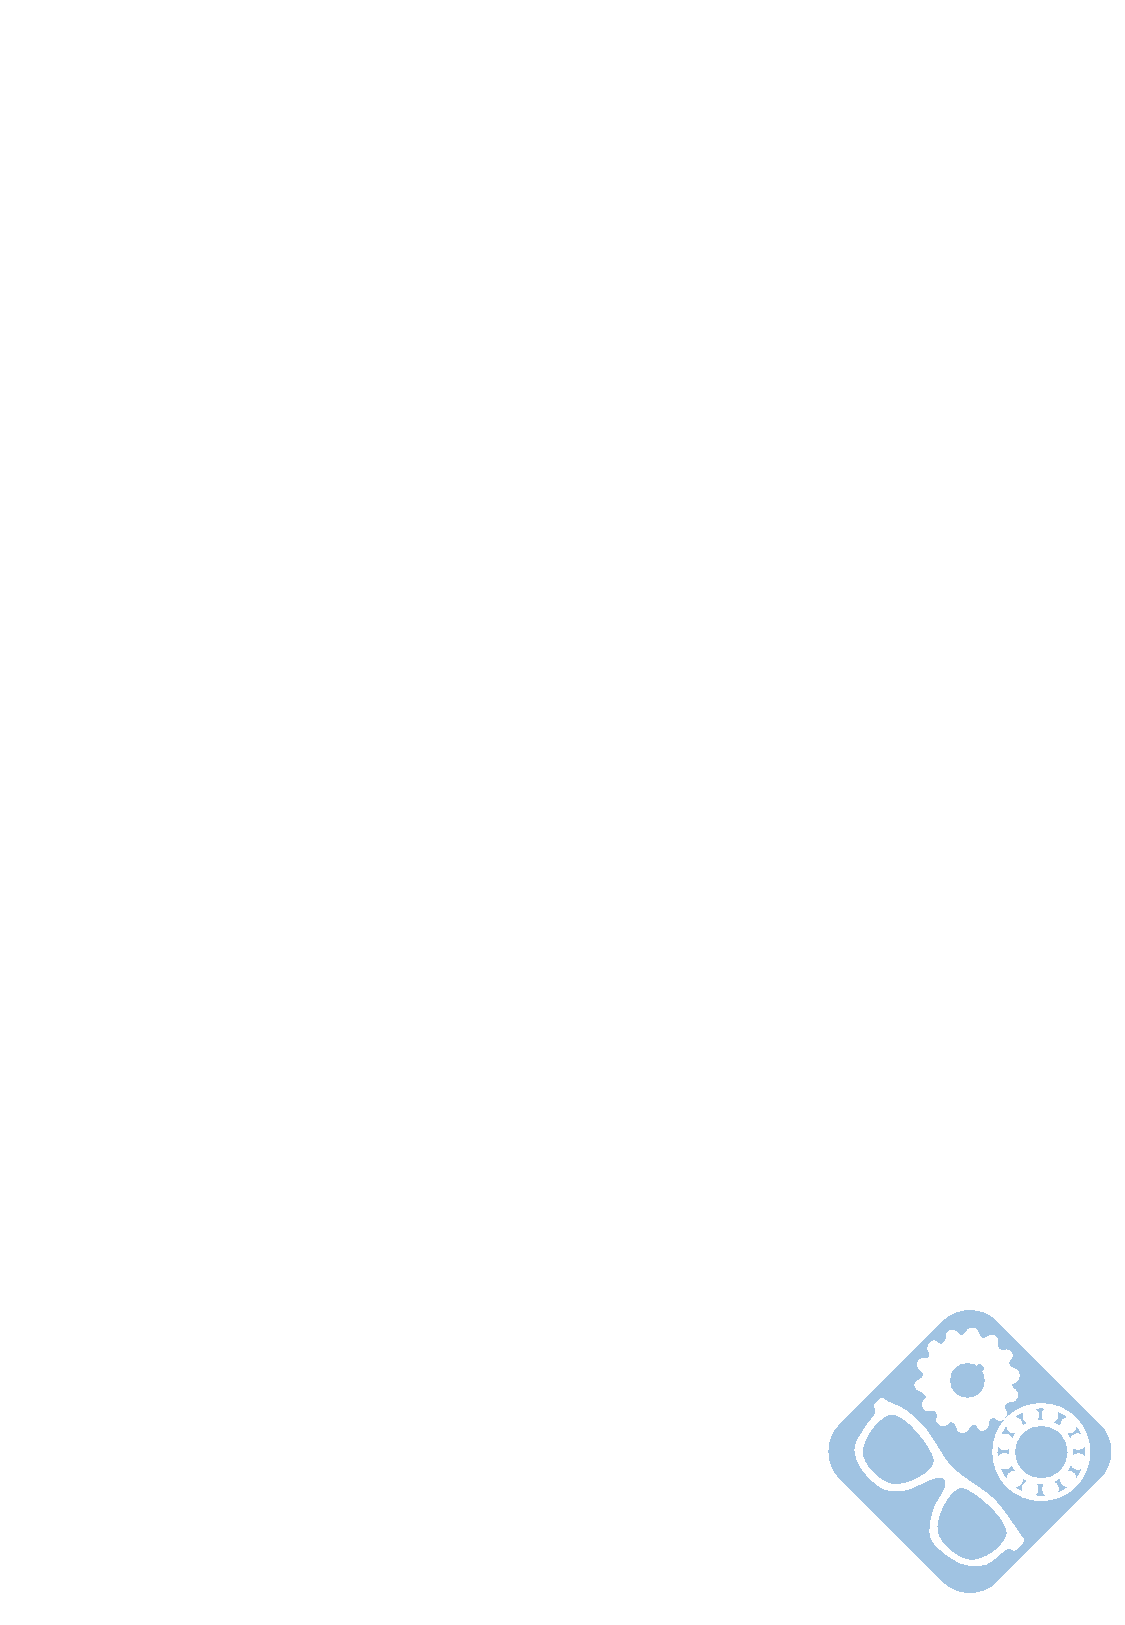
\includegraphics[width=\paperwidth,height=\paperheight,%
keepaspectratio]{../../../img/fond4}%
\end{center}
\vfill
}}}

\begin{document}

\pagestyle{empty}

\AddToShipoutPicture*{\BackgroundPic}


\includegraphics[width=2cm]{../../../img/logo}

\Huge{DS \numero - \sujet}

\vspace{1cm}

\ifdef{\prive}{\begin{center}\colorbox{danger}{\Huge{Avec Correction}}\end{center}}{}

\begin{center}
\centering\huge{PTSI}
\end{center}

\vspace{2cm}


\begin{center}
\centering\Large{\jour}
\end{center}

\vspace{2cm}

\normalsize

\tableofcontents

\newpage

\AddToShipoutPicture{\BackgroundPicdeux}

\pagestyle{fancy}

\begin{center}
\Huge \sujet
\end{center}


\normalsize


\paragraph{Contexte} ~\ \\

Le vélo Pro-Form TDF (Tour de France), étudié ici, se distingue des vélos d'appartements classiques car il permet une immersion dans un environnement réaliste. Il est ainsi possible de reproduire les tracés réels d'une étape du Tour de France. Les écrans affichent généralement le rythme cardiaque et la distance parcourue sans oublier les calories brûlées à chaque entraînement ou encore la vitesse du cycliste. Grâce à ces statistiques, il est possible de cerner les faiblesses et les forces de l'utilisateur lors d'un parcours afin de permettre une progression continue.

\posetafigure{fig01}{0.8}{Vélo Pro-Form TDF}

\paragraph{Mise en situation} ~\ \\

Ce vélo doit permettre de reproduire le plus fidèlement possible l'effort que doit fournir le cycliste en situation réelle. Vingt-quatre étapes du Tour de France ont été filmées et enregistrées avec les informations de dénivelé.
Au rythme du défilement des images, le vélo va ajuster son inclinaison ainsi que la résistance au pédalage afin d'être conforme à la sensation et l'effort réel, comme le montre la figure \ref{fig01}.

Aussi il convient d'élaborer une loi de commande du dispositif de freinage qui va dépendre de la vitesse de rotation de la roue arrière et du dénivelé de la route souhaité.

\paragraph{Objectif final} ~\ \\

Le sujet a pour but de modéliser et analyser certaines performances du vélo Pro-Form TDF. Pour cela, il comporte deux parties avec comme objectifs :
\begin{itemize}
 \item modéliser et valider le dispositif de freinage permettant de simuler la résistance au pédalage en conditions réelles,
 \item modéliser et vérifier le dimensionnement de la structure permettant d'incliner le vélo Pro-Form TDF.
\end{itemize}

\paragraph{Extrait du cahier des charges} ~\ \\

La puissance en dBm est définie comme le rapport logarithmique entre une puissance mesurée en watts et une puissance d'un milliwatt : $P_{dBm} = 10\cdot log_{10}\left(\frac{P_{mes}}{1mW}\right)$.

\posetafigure{fig02}{0.8}{Exigences extraites du cahier des charges}

\newpage

\section{Récupération du parcours virtuel sur Internet}

Le vélo Pro-Form TDF utilise la plateforme en ligne iFit.com permettant d'avoir accès à un éventail de fonctionnalités pour aider à la remise en forme (objectifs de calories, durée, distance ou puissance). Il est notamment possible de définir son propre parcours ou d'avoir accès aux cartes Google Maps à personnaliser. Il est aussi possible de télécharger des entraînements conçus pour aider à atteindre des objectifs personnels. Afin de récupérer ces données, il est nécessaire que le vélo Pro-Form TDF accède à Internet avec une connexion de qualité.

\subsection{Paramétrage et communication avec Internet}

\objectif{Paramétrer le réseau local pour connecter le vélo à Internet et y récupérer les données d'altitude nécessaires pour suivre une étape du Tour de France.}

Le vélo Pro-Form TDF doit pouvoir être utilisé à domicile. Afin de pouvoir suivre un parcours en immersion, le vélo Pro-Form TDF se connecte à Internet via une connexion Wi-Fi. La figure \ref{fig03} donne l'architecture matérielle du réseau étudié. Le masque du sous-réseau est 255.255.255.0.

\posetafigure{fig03}{0.8}{Réseau local à domicile}

\question{Compléter le diagramme de contexte du vélo Pro-Form TDF.}

\question{Compléter le diagramme des cas d'utilisation du vélo Pro-Form TDF.}

\subsection{Vérification de la qualité de connexion Wi-Fi du vélo Pro-Form TDF}

\objectif{Vérifier que le signal reçu correspond à la norme d'une liaison Wi-Fi 2,4 GHz en France et permet un fonctionnement fluide de l'immersion.}

Afin de fonctionner correctement et avec fluidité, la bande passante de la connexion avec le vélo doit au moins être de 8 MHz avec une puissance reçue supérieure à -70 dBm. De plus, la communication Wi-Fi 2,4 GHz, utilisée par le vélo Pro-Form TDF, doit respecter les critères suivants de la norme :
\begin{itemize}
 \item la communication doit se faire sur un des 13 canaux de 2,412 GHz à 2,472 GHz,
 \item les fréquences centrales des canaux sont espacées de 5 MHz,
 \item chaque canal a une bande passante maximale de 22 MHz.
\end{itemize}

La liste des canaux et fréquences associées autorisés en Wi-Fi est donnée sur la figure \ref{fig04}.

\posetafigure{fig04}{0.8}{Différents canaux utilisés par le Wi-Fi 2,4 GHz}

Le relevé spectral de la puissance du signal reçu d'une transmission Wi-Fi entre le vélo Pro-Form TDF et la Box du fournisseur d'accès à Internet de la figure \ref{fig03} est donné sur la figure du document réponse des questions \ref{q3}, \ref{q4} et \ref{q5}.

\question{Sur le document réponse, effectuer les tracés permettant d'estimer la fréquence centrale, notée $f_c$, du signal Wi-Fi reçu. Identifier le canal utilisé pour la transmission.}

\question{Sur le document réponse, effectuer les tracés nécessaires, afin de mesurer la bande passante du signal reçu et indiquer si elle respecte celle définie dans le cahier des charges.}

\question{Estimer la valeur de la puissance moyenne reçue dans la bande passante. Conclure, sous forme de tableau, sur la qualité de la connexion Wi-Fi du vélo Pro-Form TDF. Indiquer deux caractéristiques du réseau local et de la connexion qui pourraient impacter les performances de l'immersion.}

\newpage

\subsection{Récupération des données d'altitude à partir de Google Maps}

\objectif{Évaluer la possibilité de récupérer les pentes d'un parcours afin de commander le système d'inclinaison du vélo Pro-Form TDF.}

Lorsque le vélo Pro-Form TDF est connecté à Internet, grâce aux services proposés par Google, il est possible de suivre un parcours en voyant les images de la route défiler comme si l'utilisateur était sur la route avec son vélo. Le vélo utilise pour cela les API (API est un acronyme anglais qui signifie \og Application Programming Interface \fg ou Interface de Programmation d'Application) de Google et notamment l'API \verb?Elevation? qui permet de récupérer l'altitude à partir de coordonnées géographiques.

Pour cela, une requête contenant les coordonnées géographiques des différents points du parcours est utilisée.

Cette requête renvoie l'altitude de points régulièrement espacés (variable distance) le long du parcours. On s'intéresse, à titre d'exemple, à la montée du mont Ventoux en passant par Bédoin et le chalet Reynard. L'utilisateur du vélo Pro-Form TDF peut afficher le profil du parcours choisi comme illustré sur la figure \ref{fig05}.

\posetafigure{fig05}{0.6}{Profil de la montée du mont Ventoux}

Afin de commander le dispositif d'élévation du vélo Pro-Form TDF, il est nécessaire de récupérer les différentes pentes, comme illustré sur la figure \ref{fig06}.

\posetafigure{fig06}{0.6}{Pente moyenne par kilomètre lors de la montée du mont Ventoux}

\question{En utilisant les API Google, on a obtenu l'altitude d'une suite de points $P_0,P_1,...,P_n$ régulièrement espacés le long du parcours de $P_0$ à $P_n$. Écrire en Python une fonction d'entête 

\verb?def calculerPentes(distance:float, altitude:[float]) -> [float]:?

qui prend en argument la distance le long du parcours entre deux points successifs quelconques $P_i$ et $P_{i+1}$ et une liste donnant l'altitude de chaque point $P_i$. Cette fonction renvoie une liste dont l'élément d'indice $i$ donne
la pente, en pourcent, de la portion du parcours située entre les points $P_i$ et $P_{i+1}$.}

Ainsi, si la connexion Internet est bonne, il est possible de récupérer des pentes tous les 100 m le long d'un parcours ce qui permet de suivre le plus fidèlement possible le trajet sur Google Maps. Maintenant que cette information de pente est disponible, il faut la traduire en résistance au pédalage ce qui est l'objet de la prochaine partie.

\section{Résistance au pédalage}

\objectif{Modéliser l'action mécanique de résistance totale à l'avancement en fonction de la vitesse du cycliste et du dénivelé du terrain. Cette action mécanique servira au réglage de la résistance au pédalage du vélo Pro-Form TDF.}

En cyclisme, différentes forces, appelées résistances ici, s'opposent à l'avancement du cycliste et limitent sa vitesse de déplacement. À vitesse élevée ($>40km\cdot h^{-1}$), la résistance aérodynamique est la plus importante de toutes ces forces. Pour se représenter son importance, il faut savoir que 90\% de la puissance produite par un cycliste sert à vaincre cette résistance sur un terrain plat.

La résistance à l'avancement de l'ensemble cycliste-vélo, se décompose en trois termes (figure \ref{fig07}):
\begin{itemize}
 \item la résistance due à la gravité qui s'exerce sur l'ensemble cycliste-vélo $\vec{R}_G$,
 \item la résistance due à la friction $\vec{R}_R$,
 \item la résistance aérodynamique $\vec{R}_A$.
\end{itemize}

Ainsi la résistance totale à l'avancement $\vec{R}_T$ est donnée par $\vec{R}_T=\vec{R}_A+\vec{R}_R+\vec{R}_G$.

Données :
\begin{itemize}
 \item $\vec{R}_R=-R_R\cdot\vec{x}_1$, 
 \item $\vec{R}_G=-R_G\cdot\vec{x}_1=-M\cdot g\cdot sin\left(\theta\right)\cdot\vec{x}_1$,
 \item $\vec{P}=M\cdot\vec{g}$, avec $M$ la masse totale de l'ensemble cycliste-vélo.
 \end{itemize}

\posetafigure{fig07}{0.5}{Modélisation de la résistance au pédalage}

\newpage

\subsection{Modélisation de la résistance au pédalage}

La résistance à la friction $R_R=C_R\cdot M\cdot g$ dépend du contact des roues avec le terrain sur lequel évolue le cycliste.

$C_R$ dépend essentiellement de la pression de gonflage des pneumatiques ($P_R$ en kPa), des matériaux composant les pneumatiques et de la nature du terrain. Le graphique de la figure \ref{fig08} donne l'évolution de $C_R$ (sans unité)
en fonction de la pression $P_R$.

\posetafigure{fig08}{0.6}{Coefficient de roulement}

\question{Relever la valeur de $C_R$ pour une pression de pneumatique de 950 kPa.}

~\

La résistance aérodynamique $R_A$ est directement proportionnelle à l'aire frontale projetée du cycliste et de son vélo ($A_p$ en $m^2$), au coefficient de trainée ($C_D$ sans unité), à la masse volumique de l'air ($\rho$ en $kg\cdot m^{-3}$) et au carré de la vitesse d'écoulement de l'air sur le corps du cycliste ($v$ en $m\cdot s^{-1}$) : $R_A=-\vec{R}_A\cdot \vec{x}_1$.

$R_A=0.5\rho A_p C_D v^2$ avec $\rho=1.293e^{-0.124h}\frac{273}{T}$ où $T$ est la température en kelvins et $h$ l'altitude du cycliste en km. On donne $e^{-0.124\times 2.25}\approx 0.75$.

\question{Calculer $R_A$ pour $A_p C_D=0.22m^2$, $v=15m\cdot s^{-1}$, une température de 293K (soit 20 °C) et les altitudes de 0 km et de 2,25 km. Conclure sur l'effet de l'altitude sur la résistance aérodynamique et sur le fait que le vélo
ne tient pas compte de cette donnée. Faire les approximations nécessaires.}

\question{Donner l'expression totale de $R_T$.}

~\

Plusieurs essais, rassemblés sur la figure \ref{fig09}, ont été réalisés sur une piste horizontale ($\theta=0$) à une altitude de 0 km, une température de 293K (20\degree C) et une pression des roues $P_R$ de 950 kPa.

\posetafigure{fig09}{0.35}{Résistance à l'avancement}

\vspace{-0.5cm}

\question{Justifier la forme obtenue sur la figure \ref{fig09}. Recaler la valeur du coefficient $A_p C_D$ à partir des essais de cette figure.}

~\

Le modèle obtenu a permis de tracer les graphiques de la figure \ref{fig10}.

\posetafigure{fig10}{0.7}{Courbe obtenue à partir du modèle}

\question{Conclure sur la résistance maximale à l'avancement que le vélo Pro-Form TDF doit restituer à l’utilisateur.}

~\

Le modèle ainsi obtenu constitue la loi de commande du dispositif de freinage du vélo Pro-Form TDF. La partie suivante du sujet va permettre d'étudier la manière dont cet effort est réalisé et piloté.

\subsection{Dispositif de freinage}

\objectif{Vérifier la capacité du vélo Pro-Form à restituer la sensation de résistance totale à l’avancement et déterminer la commande de déplacement nécessaire au niveau des aimants du dispositif de freinage.}

La partie précédente a permis de mettre en évidence la résistance totale à l’avancement $R_T$ (en N) que le cycliste doit vaincre pour avancer. Afin que la sensation soit la plus proche possible de la réalité, un dispositif de freinage
magnétique exerce un moment de freinage, noté $M_f$ (en $N\cdot m$), sur la roue arrière du vélo d’appartement. Pour cela, le moment de freinage doit respecter la relation suivante : $R R_T=M_f$ avec $R$(35 cm) le rayon de la roue d’un vélo réel et $R_T$ la résistance totale à l’avancement.

\posetafigure{fig11}{0.8}{Mesure et modélisation du couple de pédalage}

La roue arrière du vélo d’appartement est assimilée à un disque métallique de rayon $R_d$ (15 cm), d’épaisseur $e$ (5 mm), de conductivité $\gamma$ et tournant à une vitesse angulaire $\omega$. Quatre aimants sont placés de chaque côté
de la roue arrière. Afin de simplifier l’étude, les quatre aimants sont assimilés à deux aimants produisant un champ magnétique $\vec{B}$ quasi-uniforme perpendiculaire au disque sur un secteur d’angle $\alpha$ situé entre un rayon $R_1$ variable et $R_2=R_d$. Le rayon $R_1$ dépend de la position verticale des aimants $\Delta_y$. L’angle $\alpha$ est supposé constant.

\posetafigure{fig12}{0.4}{Dispositif de freinage}

Un élément de volume, noté $dV=e\cdot dS=erdrd\theta$, de la roue arrière est repéré par $\overrightarrow{OP}=r\cdot \vec{x}_2$. La force volumique de Laplace, notée $\vec{f}_L(r)$, s’exerçant sur un élément de volume $dV$ est $\vec{f}_L(r)=\dfrac{d\vec{F}_L}{dV}=-\gamma r \omega B^2\vec{y}_2$. Le moment résultant des actions de Laplace au point $O$ se détermine à partir de la relation

\begin{center}
$\vec{M}_{O,\vec{f}_L}=\int_{secteur} \overrightarrow{OP}\wedge \vec{f}_L(r)dV$
\end{center}

\question{Déterminer le moment résultant $\vec{M}_{O,\vec{f}_L}$, l’expression de la norme du moment de freinage, notée $M_f$. Indiquer à quel type de frottement peut être assimilé ce moment de freinage et s’il peut stopper complètement la roue arrière.}

~\

Le modèle pour la résistance totale à l’avancement est donné figure \ref{fig10}.

A $25km\cdot h^{-1}$, $M_f=-\vec{M}_{O,\vec{f}_L}\cdot \vec{z}_1=0.00038(R_d^4-R_1^4)$ (rayons en mm). La caractéristique de freinage pour une vitesse de translation de $25km\cdot h^{-1}$ est donnée figure \ref{fig13}.

\posetafigure{fig13}{0.65}{Norme du moment de freinage $M_f$ pour $v=25km\cdot h^{-1}$}

\question{En déduire le déplacement $\Delta_y$ nécessaire des aimants pour assurer la résistance maximale $R_T$ à l’avancement de la figure \ref{fig10}.}

~\

Cette étude a donc permis de faire le lien entre la résistance à l’avancement en situation réelle et le déplacement $\Delta_y$ d’un aimant qui permet de reproduire cet effort sur un vélo d’appartement. La partie suivante permet d’étudier la manière dont est généré et piloté ce déplacement.

\subsection{Pilotage du dispositif de freinage}

\objectif{Linéariser le modèle entre le déplacement des aimants et la commande du mécanisme de déplacement.}

\posetafigure{fig14}{0.7}{Modèle et paramétrage du système de freinage}

\question{À partir du modèle figure \ref{fig14} et à l’aide d’une fermeture géométrique, déterminer une relation sous la forme $f(\theta_3,\theta_5)=0$.}

~\

La résolution numérique de l’équation précédente est réalisée en Python. Le déplacement des aimants étant proportionnel à $\theta_5$, il est possible de tracer l’évolution du déplacement des aimants en fonction de l’angle de commande du servomoteur $\theta_3$. Le résultat de la résolution est donné sur la courbe figure \ref{fig15}.

\posetafigure{fig15}{0.5}{Loi entrée sortie}

\question{Proposer, en vous aidant des figures \ref{fig15} et \ref{fig13}, un modèle linéaire entre la norme du moment de freinage $M_f$ en $N\cdot m$ et l’angle de commande $\theta_3$ en degrés pour une vitesse de $25km\cdot h^{-1}$.}

\section{Contrôle du freinage - Modélisation et réglage de la boucle de
position}

Le contrôle de la résistance au pédalage se fait en contrôlant la position des biellettes.

\objectif{Modéliser puis régler le correcteur de l’asservissement de position des biellettes permettant un contrôle du dispositif de freinage.}

Afin de suivre le plus fidèlement possible le parcours souhaité, il est nécessaire de contrôler parfaitement la position des biellettes du dispositif de freinage. Pour cela, un asservissement de position est réalisé. La structure de cet asservissement est représentée figure \ref{fig16}.

\posetafigure{fig16}{1}{Structure de l’asservissement de position des biellettes}

Hypothèses et notations:
\begin{itemize}
 \item le réducteur est un réducteur roue et vis sans fin, défini par son rapport de réduction $K_{red}=\dfrac{\omega_3}{\omega_m}=\dfrac{1}{220}$,
 \item la mesure de position en sortie du réducteur roue et vis sans fin, notée $\theta_3(p)$, est réalisée par un potentiomètre linéaire de $10k\Omega$, alimenté en 2,2V et d’une course de 160\textdegree,
 \item la tension image de la position $\theta_3(p)$ est ensuite numérisée par un convertisseur analogique-numérique (CAN) 10bits unipolaire, codé en binaire naturel et alimenté en 0-2,2V,
 \item le couple résistant ramené sur l’axe moteur est considéré comme négligeable.
\end{itemize}

\newpage

Le schéma-bloc de l’asservissement est donné sur la figure \ref{fig17}.

\posetafigure{fig17}{1}{Schéma-bloc de l’asservissement de $\theta_5(p)$ à $\theta_c(p)$}

\question{Déterminer les valeurs numériques de $K_{CAN}$ et $K_{pot}$ modélisant respectivement le CAN et le potentiomètre. En déduire la valeur de $K_a$ en $rad^{-1}$.}

~\

Le variateur de vitesse associé au moteur est un hacheur quatre quadrants, alimenté par une tension $U_0=12V$, dont la structure de commande est représentée figure \ref{fig18}.

La loi de commande est élaborée à partir d’un rapport cyclique, noté $\alpha$, compris entre 0 et 255 incréments, et d’un signal, non étudié ici, permettant de déterminer le sens de rotation souhaité. Dans l’étude suivante, les interrupteurs $T_1-D_1$ et $T_4-D_4$ sont commandés pour $t\in \left[0,\frac{\alpha}{255}T_d\right[$ puis $T_1-D_1$ et $T_2-D_2$ pour $t\in \left[\frac{\alpha}{255}T_d,T_d\right[$. Le chronogramme de la tension moteur correspondant est donné figure \ref{fig18}.

\posetafigure{fig18}{1}{Structure de commande et exemple de tension moteur $u_m$.}

La période de découpage est notée $T_d$. La résistance $R_m$, l’inductance $L_m$ et la force électro-motrice $e(t)$ modélisent le moteur qui est une machine à courant continu à aimants permanents.

\question{Justifier l’intérêt d’une telle structure de commande pour la commande du moteur du dispositif de freinage.}

\question{Déterminer la relation entre la valeur moyenne de $u_m$, notée $\langle u_m(t)\rangle$, $\alpha$ et $U_0$, puis tracer $\langle u_m(t)\rangle$ en fonction du rapport cyclique $\alpha$.}

\question{En déduire l’expression du gain $K_v$ sachant que dans le modèle adopté 
$L(\langle u_m(t)\rangle)=U_m(p)$.}

\question{Indiquer la non linéarité qui pourrait être prise en compte dans le schéma-bloc afin de modéliser le comportement du hacheur.}

~\

Un essai est réalisé en boucle ouverte, en imposant au moteur une variation en échelon au niveau du rapport cyclique $\alpha(p)$ de 50 incréments (le rapport cyclique est compris entre 0 et 255 incréments) à l’instant $t=0,5$s.

La mesure de vitesse en sortie du moteur se fait à l’aide d’une génératrice tachymétrique modélisée par un gain de $0,12V\cdot s$ comme indiqué sur la figure \ref{fig19}. L’allure de la réponse à l’essai est donnée sur la figure B du
document réponse.

\posetafigure{fig19}{0.6}{Schéma-bloc de la mesure en boucle ouverte}

\question{Identifier un modèle, en détaillant les méthodes utilisées pour identifier les paramètres, et en réalisant les tracés sur la figure du document réponse, pour la fonction de transfert $\frac{U_v(p)}{\alpha(p)}$. En déduire la fonction de
transfert $H_v(p)=\frac{\omega_m(p)}{\alpha(p)}$.}

Remarque : $H_v(p)=K_v\cdot H_m(p)$.

~\

Le correcteur est un correcteur proportionnel de valeur $C(p)=K_c$.

\question{Déterminer l’expression de la fonction de transfert en boucle ouverte donnée figure \ref{fig17}, puis justifier que le critère de précision du cahier des charges est respecté.}

\question{Déterminer, en réalisant les tracés sur la figure du document réponse, la fonction de transfert en boucle ouverte $H_{BO}(p)$ pour $K_c=1$.}

~\

Pour la suite, on prendra $H_{BO}(p)=\frac{0.76}{p\left(1+\frac{p}{10}\right)}$ pour $K_c=1$.

\question{Exprimer la fonction de transfert en boucle fermée $H_{BF}(p)=\frac{\theta_3(p)}{\theta_c(p)}$ et exprimer ses paramètres caractéristiques, son gain statique $K_{BF}$, sa pulsation propre $\omega_{0BF}$ et son amortissement $\xi_{BF}$.}

~\

L’abaque du temps de réponse réduit en fonction de l’amortissement est donné sur la figure \ref{fig20}.

\question{Déterminer la valeur limite du correcteur proportionnel permettant de satisfaire le critère de dépassement du cahier des charges et reporter la valeur dans le tableau du document réponse de la question \ref{q27}.}

\question{Déterminer la valeur limite du correcteur proportionnel permettant de satisfaire le critère de rapidité du cahier des charges et reporter la valeur dans le tableau du document réponse de la question \ref{q27}. Cette valeur est à déterminer en exploitant le diagramme de Bode de la FTBO.}

\question{Conclure sur la plage de valeur du correcteur proportionnel qui permettrait de respecter tous les critères du cahier des charges en complétant le tableau du document réponse. Vous Identifierez $K_{cmin}$ et $K_{cmax}$ sur le tracé du document réponse.}

\posetafigure{fig20}{0.6}{Abaque du temps de réponse réduit en fonction de l’amortissement}

\section{Étude du dispositif d'inclinaison}

\subsection{Problème de non basculement du vélo Pro-Form TDF}

\objectif{L’objectif de l’étude est de vérifier que les dimensions du vélo sont suffisantes afin que celui-ci ne bascule pas lorsque le cycliste se met en danseuse.}

Lors de l'ascension d'un col ou tout simplement en montée le vélo va s'incliner et la résistance va augmenter. Afin de moins solliciter les muscles des cuisses, le cycliste va se mettre en danseuse c'est à dire qu'il va translater son bassin afin de le mettre à la verticale de la pédale sur laquelle il faut effectuer un effort. Ainsi, le poids de son corps va l'aider à effecteur le mouvement. Le mouvement du bassin va engendrer un transfert de masse sur les appuis qui peut occasionner un décollement.

\newpage

Le schéma qui permet de faire l'étude de modélisation plane est donné figure \ref{fig21}. Il est composé de 3 ensembles :
\begin{itemize}
 \item le sol 0 qui est le référentiel galiléen,
 \item le vélo 1 qui est immobile par rapport au sol. Il est en appui sur deux liaisons sphères/plans avec frottement en D et en E. Il a une masse $m_1$ et de centre de gravité $G_1$,
 \item le cycliste $c$ de masse $m$ et un centre de gravité $G$. Pour cette étude, le mouvement du cycliste est une translation rectiligne suivant $\vec{z}$ qui correspond au mouvement du bassin : $\vec{\gamma}_{G\in c/0}=\gamma\vec{z}$.
\end{itemize}

~\

$\overrightarrow{AG}=b\vec{y}+c(t)\vec{z}$, $\overrightarrow{AD}=-e\vec{y}+d\vec{z}$, $\overrightarrow{AE}=-e\vec{y}-d\vec{z}$, $\overrightarrow{AG_1}=h\vec{y}$.

~\

Les seules actions mécaniques à prendre en compte sont :

\begin{minipage}{0.49\linewidth}
$\left\{Td_{0\rightarrow 1}\right\}=\left\{\begin{array}{c}
N_D\vec{y}+T_D\vec{z}\\\vec{0}\end{array}\right\}_D$

$\left\{Te_{0\rightarrow 1}\right\}=\left\{\begin{array}{c}
N_E\vec{y}+T_E\vec{z}\\\vec{0}\end{array}\right\}_E$
\end{minipage}\hfill
\begin{minipage}{0.49\linewidth}
$\left\{T_{pes\rightarrow 1}\right\}=\left\{\begin{array}{c}
-m_1g\vec{y}\\\vec{0}\end{array}\right\}_{G_1}$

$\left\{T_{pes\rightarrow 1}\right\}=\left\{\begin{array}{c}
-mg\vec{y}\\\vec{0}\end{array}\right\}_G$.
\end{minipage}

~\

Lors de la décélération ($\gamma<0$), il y a un transfert de masse qui peut engendrer le décollement au point E.

\question{Faire un graphe des liaisons et des actions mécaniques. Le graphe ne comporte que deux ensembles $\left\{0\right\}$ et $\left\{1+c\right\}$.}

~\

L'application du Principe Fondamental de la Dynamique permet de montre que :

$\overrightarrow{\delta_{D,c/0}}=\overrightarrow{M_{D,O_D\rightarrow 1}}+\overrightarrow{M_{D,O_E\rightarrow 1}}+\overrightarrow{M_{D,p\rightarrow c}}+\overrightarrow{M_{D,p\rightarrow 1}}=(b+e)\cdot m\cdot\gamma\cdot \vec{x}$.

\question{Indiquer, puis appliquer une stratégie d'isolements permettant de déterminer $N_E$ en fonction de $b$, $e$, $m$, $\gamma$, $d$, $m_1$, $g$, $c$.}

~\

On rappelle qu'à la limite du basculement, $N_E=0$.

\question{Calculer $\gamma$, l'accélération transversale, pour faire basculer le vélo et conclure sur l'exigence id=1.1. $m_1=56kg$, $=125kg$, $d=0.25m$, $c=0.2m$, $h=0.35m$, $e=0.05m$, $b=1.1m$ et $g=9.81m\cdot s^{-2}$.}

\posetafigure{fig21}{0.8}{Modélisation adoptée pour l’étude du basculement}

\newpage

\subsection{Dimensionnement du vérin}

\objectif{L’objectif est de valider le dimensionnement du vérin qui permet d’incliner le vélo pour un rendu plus réaliste.}

\posetafigure{fig22}{1}{Inclinaison}

\question{Déterminer $\vec{V}_{B\in 1/0}$ en fonction de $R$, $\dot{\theta}_1$ et $\vec{V}_{B\in 2/0}$ en fonction de $\dot{\lambda}$, $\lambda$ et $\dot{\theta}_2$.}

\question{Montrer que $\dot{\lambda}=-R\dot{\theta}_1\cdot cos(\theta_2-\theta_1)$.}

\question{Sachant que le cahier des charges impose une vitesse de rotation $\dot{\theta}_1=0.023rad\cdot s^{-1}$ et que $R=250mm$ en déduire la vitesse maximale de la tige du vérin.}

~\

Dans le pire des cas, le vérin électrique doit générer en régime permanent un effort de 1500 N à une vitesse de sortie de tige de $5,2mm\cdot s^{-1}$. Il a un rendement de 0,3. Il est alimenté en monophasé 120 V, 50 Hz avec un courant maximal de 0,5 A et un facteur de puissance de $cos\varphi=0,8$. On rappelle que la puissance fournie vaut $P_{fmax}=U\cdot I_{max}\cdot cos\varphi$.

\question{Déterminer la puissance à fournir en régime permanent. Conclure sur la capacité de l’actionneur à pouvoir incliner le vélo pour suivre les étapes du Tour de France.}

\section{Synthèse}

Un vélo d’appartement classique ne dispose ni du système d’inclinaison, ni de l’immersion avec Google Maps permettant de suivre les différentes étapes du Tour de France.

\question{Remplir le tableau du document réponse, en indiquant si les exigences du cahier des charges sont vérifiées et en précisant la démarche utilisée pour les vérifier.}

\question{Remplir le tableau du document réponse, afin de comparer le vélo Pro-Form TDF avec un vélo d’appartement traditionnel en citant les avantages et les inconvénients apportés par chacun d’eux du point de vue immersion et complexité.}

\begin{center}
\Large{FIN}
\end{center}

\cleardoublepage

\ifdef{\public}{\pagestyle{docreponse}}{\pagestyle{correction}}

\reponse{0}{\begin{center}
  \def\svgwidth{.6\textwidth}
  \input{img/DR01.pdf_tex}
\end{center}}{\begin{center}
  \def\svgwidth{.6\textwidth}
  \input{img/DR01_cor.pdf_tex}
\end{center}}

\reponse{0}{\begin{center}
  \def\svgwidth{.6\textwidth}
  \input{img/DR02.pdf_tex}
\end{center}}{\begin{center}
  \def\svgwidth{.6\textwidth}
  \input{img/DR02_cor.pdf_tex}
\end{center}}

\reponse{2}{\begin{center}
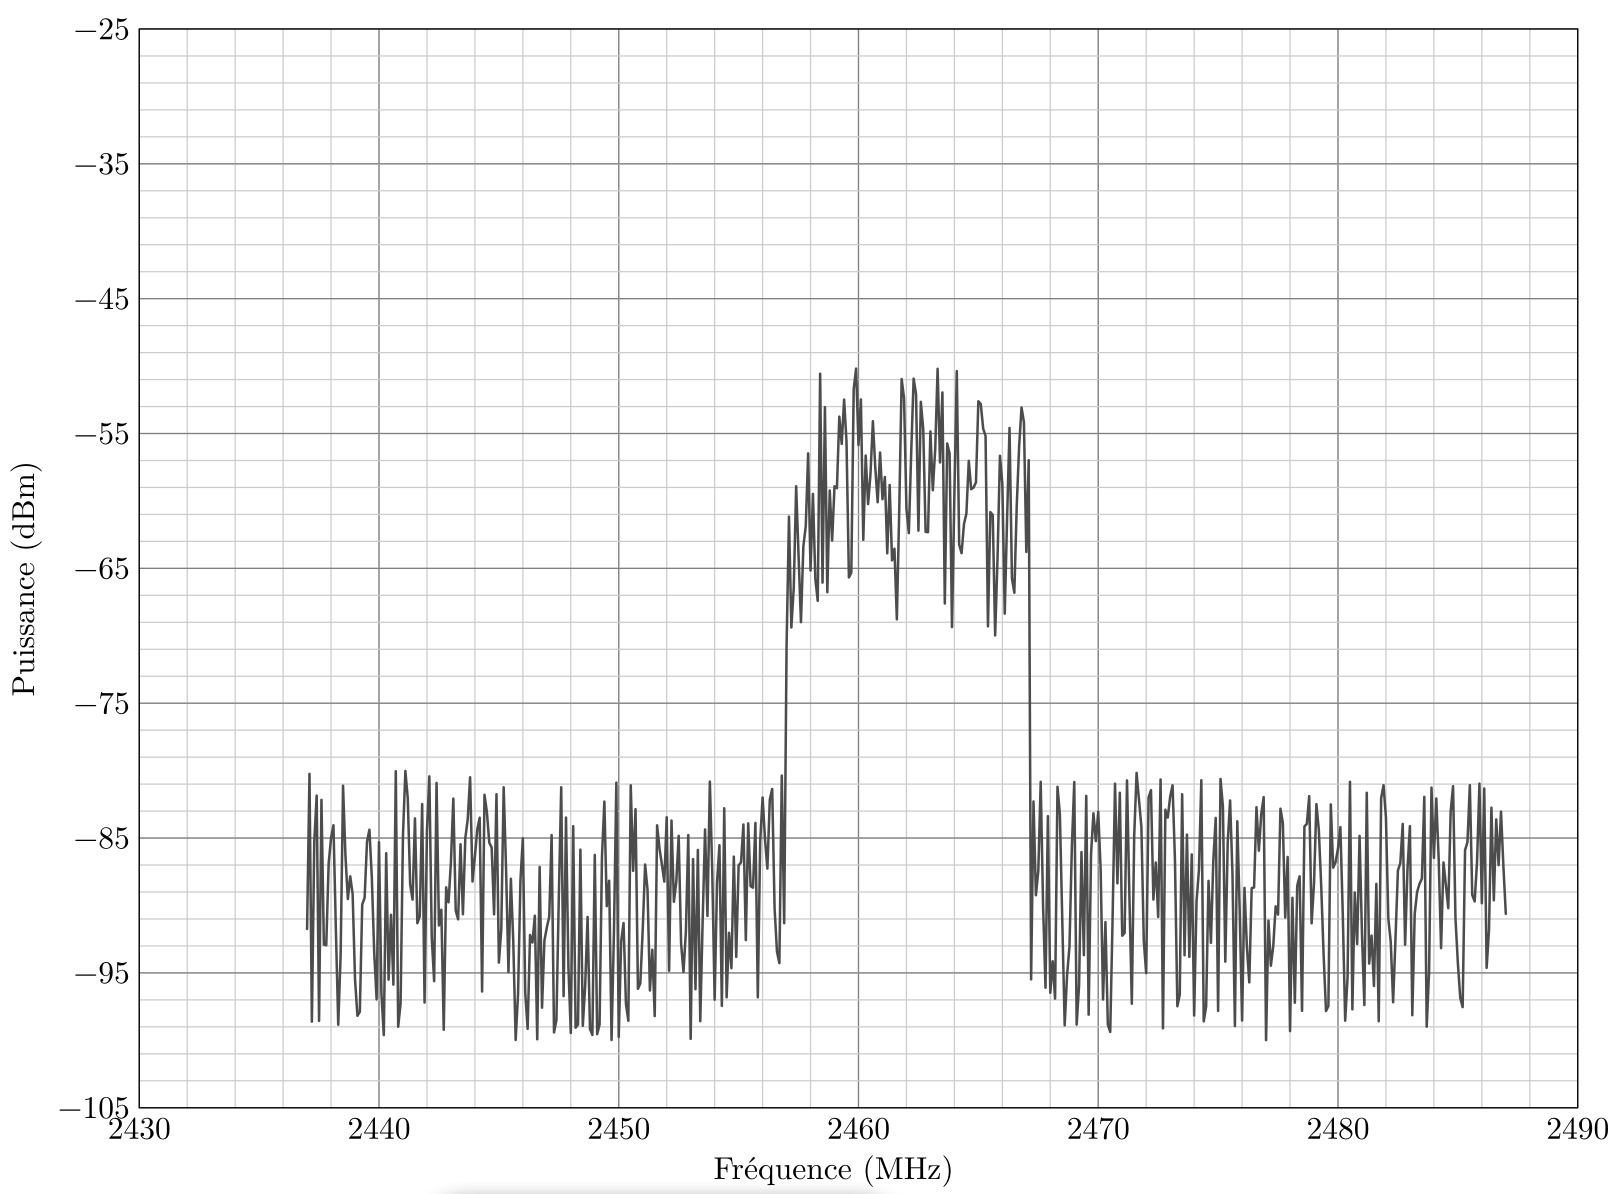
\includegraphics[width=0.5\linewidth]{img/DR03}
\end{center}}{\begin{center}
  \def\svgwidth{.5\textwidth}
  \input{img/DR03_cor1.pdf_tex}
\end{center}
C'est le canal 11.}

\reponse{2}{\begin{center}
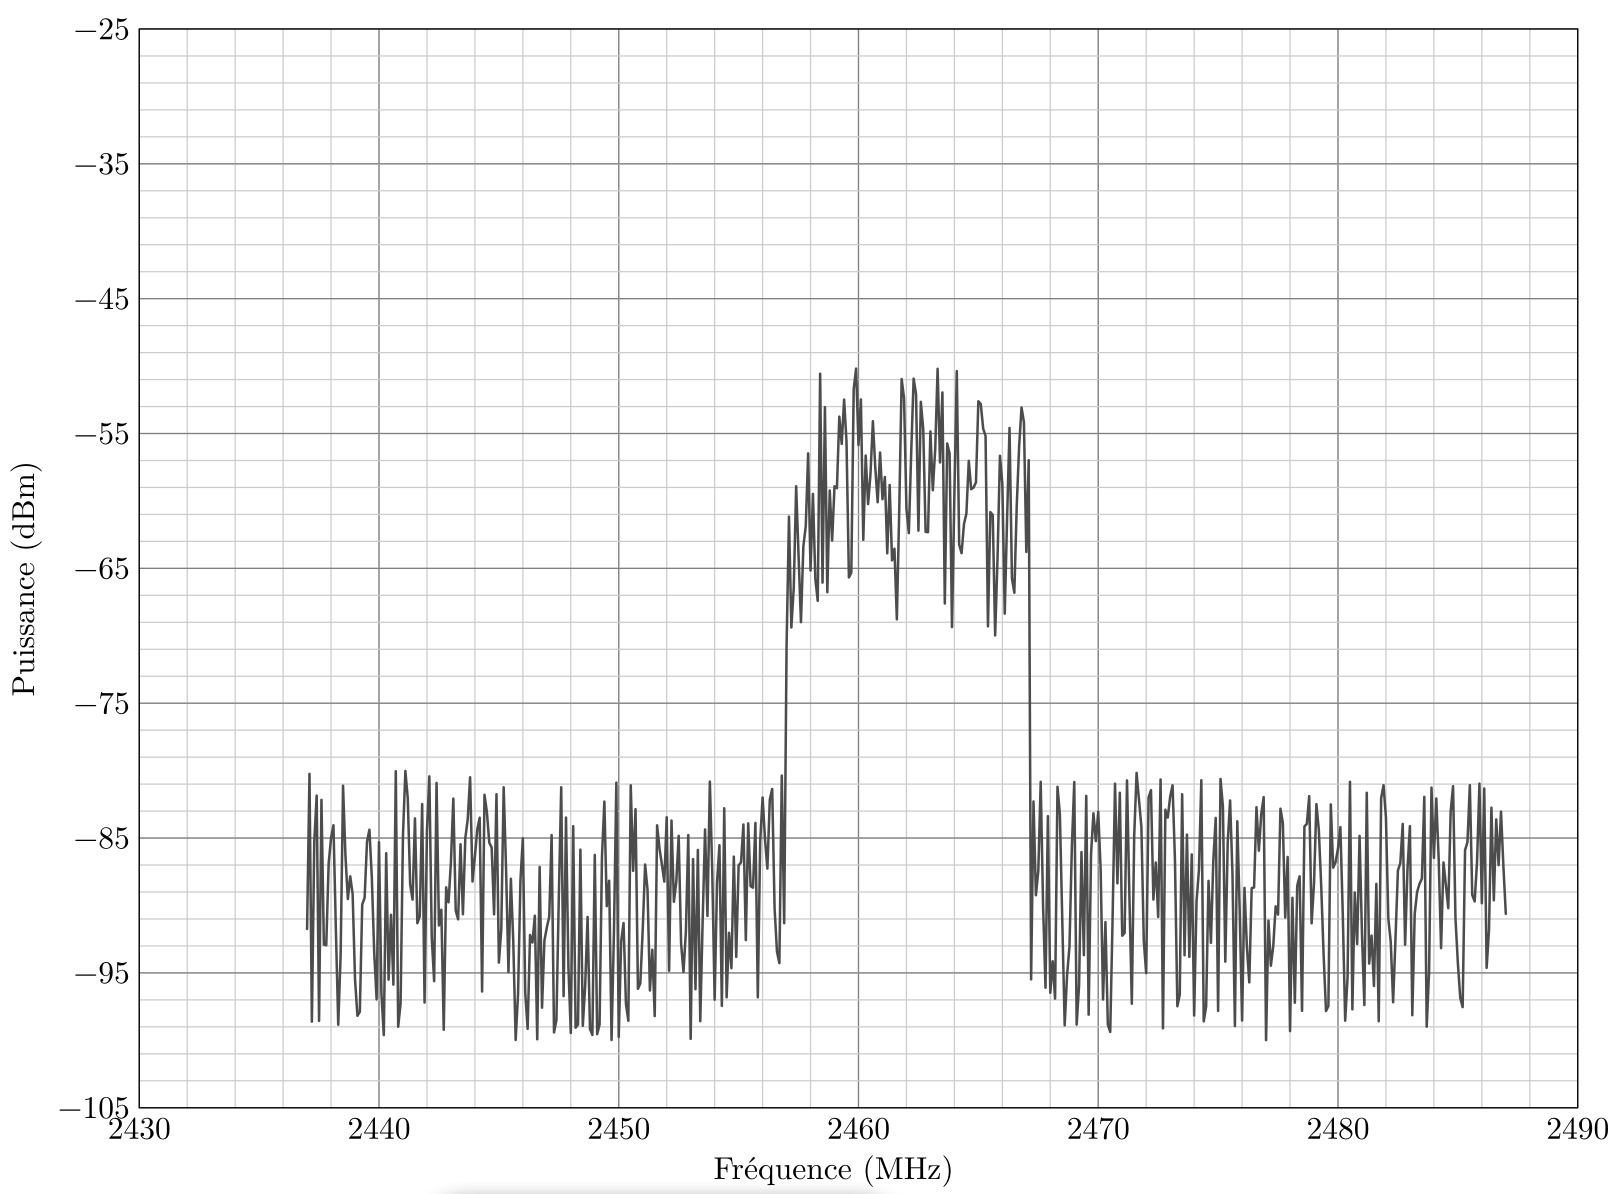
\includegraphics[width=0.5\linewidth]{img/DR03}
\end{center}}{\begin{center}
  \def\svgwidth{.5\textwidth}
  \input{img/DR03_cor2.pdf_tex}
\end{center}}

\reponse{2}{\begin{center}
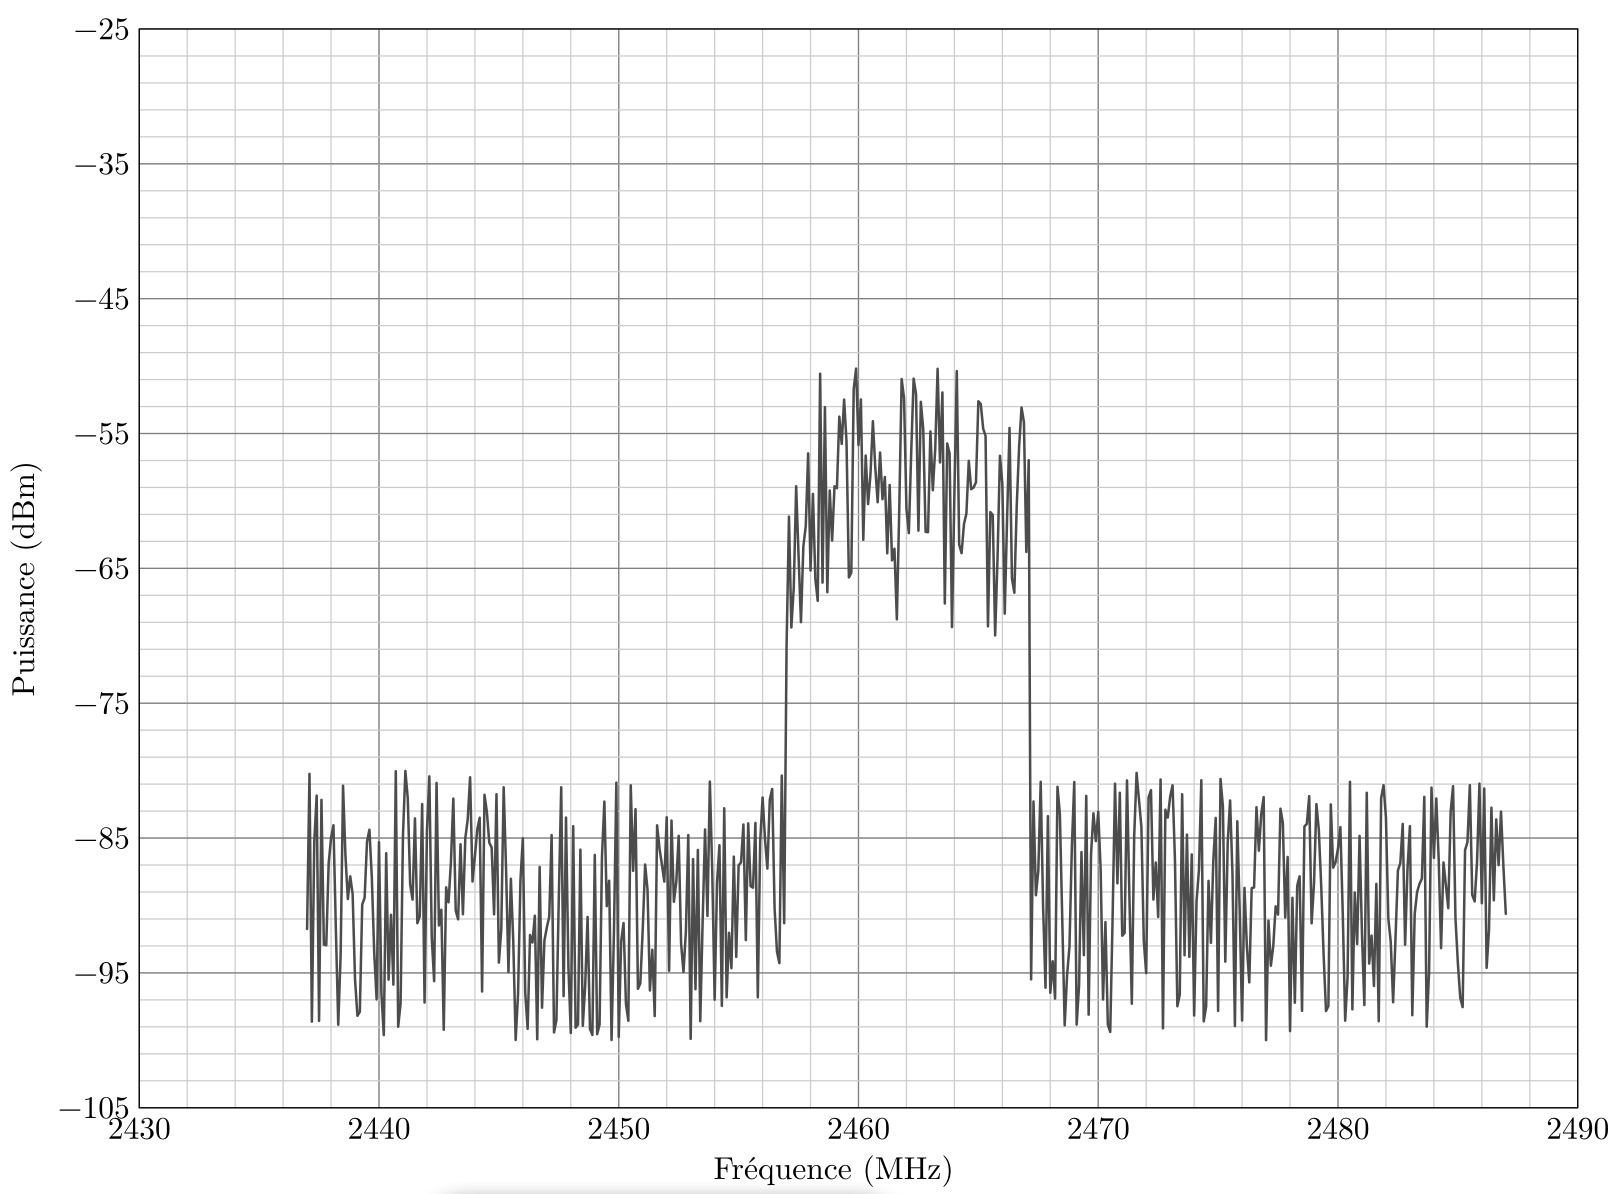
\includegraphics[width=0.5\linewidth]{img/DR03}

\begin{tabular}{|c|c|c|c|}
\hline
& Fréquence (en $GHz$) & Puissance & $\Delta BP$ \\
\hline
Cahier des charges & & & \\
\hline
Valeur mesurée & & & \\
\hline
Bilan & & & \\
\hline
\end{tabular}
\end{center}
}{\begin{center}
\def\svgwidth{.5\textwidth}
  \input{img/DR03_cor3.pdf_tex}

\begin{tabular}{|c|c|c|c|}
\hline
& Fréquence (en $GHz$) & Puissance & $\Delta BP$ \\
\hline
Cahier des charges & $2,412$ à $2,472$ & $>-70dBm$ & $>8MHz$ $<22MHz$ \\
\hline
Valeur mesurée & $2,462GHz$ & $-60dBm$ & $10MHz$ \\
\hline
Bilan & Respecté & Respecté & Respecté \\
\hline
\end{tabular}
\end{center}

Caractéristiques du réseau local et de la connexion qui pourraient impacter
les performances de l’immersion:
\begin{itemize}
 \item Trop de débit dans le réseau local et éloignement du vélo avec la box,
 \item Connexion internet : débit de la connexion.
\end{itemize}}

\newboolean{printdr}
\newboolean{printcor}
\setboolean{printdr}{false}
\setboolean{printcor}{false}

\reponse{0}{\setboolean{printdr}{true}}{\setboolean{printcor}{true}}


\ifprintcor
\begin{minted}[xleftmargin=2em,linenos,firstnumber=1]{python}
def calculerPentes(distance,altitude):
	n = len(altitude)
	Ls = [0] * (n-1)  # n-1 pentes entre n altitudes
	for i in range(n-1):
		Ls [i] = (altitude[i+1]-altitude[i])/distance
	return Ls
\end{minted}
\fi

\ifprintdr
\begin{minted}[xleftmargin=2em,linenos,firstnumber=1]{python}







\end{minted}
\fi

\reponse{2}{}{\begin{center}
  \def\svgwidth{.5\textwidth}
  \input{img/fig08_cor.pdf_tex}
\end{center}
}

\reponse{4}{}{
\begin{itemize}
 \item Pour $h=0$, $R_A=0.5\times 1.3 \times 0.2 \times 15^2=13 \times 1.5\times 1.5=(13+6.5)\times 1.5=(19.5+9.75)=29.25N$,
 \item Pour $h=2.25$, $R_A=0.5\times 1.3 \times 0.2 \times 0.75 \times 15^2=29.25\times 0.75=29.25-7,3=22N$
\end{itemize}

On a donc : $\dfrac{\Delta R_A}{R_A}=\dfrac{29.25-22}{29.25}=\dfrac{7.25}{29.25}\approx 25\%$. Cette variation n'est pas négligeable mais la variation est très progressive et $R_A$ dépend surtout de la vitesse.}

\reponse{2}{}{$R_T=(C_R+sin\theta)Mg+0.5\cdot\rho A_d\cdot C_D\cdot v^2$}

\reponse{4}{}{Sur la figure, on trouve $R_T=\alpha\cdot v^2+R_{T0}$

Avec $\alpha=\dfrac{17-2.5}{80}=\dfrac{14.5}{80}\approx 0.2$,
donc $0.5\cdot\rho\cdot A_d\cdot C_D=0.2$, donc $A_d\cdot C_D=\dfrac{0.2}{0.5\cdot 1.3}=\dfrac{0.2}{0.65}\approx 0.3m^2$}

\reponse{3}{}{On donne $RT_{max}=60N$. D'après la figure 10, on constate que l'effort dépend bien de la vitesse jusqu'à 4° la plage en saturation ne sera pas utile car la vitesse de $30km\cdot h^{-1}$ semble inatteignable sur une telle pente. Par contre à partir de 5°, il n'y a plus de variation possible.}

\reponse{6}{}{
$\vec{M}_{O,\vec{f}_L}=\int_{secteur} r\cdot \vec{x}_2\wedge (-\gamma r \omega B^2\vec{y}_2)erdrd\theta$

$\vec{M}_{O,\vec{f}_L}=-\gamma\cdot \omega\cdot B^2\cdot e\cdot \vec{z}_2\int_{r=R_1}^{r=R_2} r^3\cdot dr\int_{\theta=0}^{\theta=\alpha}d\theta=-\gamma\cdot r\cdot \omega\cdot B^2\cdot e\cdot \vec{z}_2\left[\dfrac{r^4}{4}\right]_{r=R_1}^{r=R_2} \alpha=-\gamma\cdot r\cdot \omega\cdot B^2\cdot e\cdot  \alpha\dfrac{R^4_2-R^4_1}{4}\cdot \vec{z}_2$

Donc, $Mf=\gamma\cdot r\cdot \omega\cdot B^2\cdot e\cdot  \alpha\dfrac{R^4_2-R^4_1}{4}$, c'est proportionnel à $\omega$, il s'agit donc de frottement visqueux, il ne peut pas stopper la roue car ce freinage tend vers 0 quand la vitesse tend vers 0.}

\reponse{3}{}{$R_{Tmax}=60N$, or $Mf_{max}=R\cdot R_{Tmax}=0,35\times 60=21N\cdot m$.

Sur la courbe, on lit donc $\Delta y=0.0195m$.}

\reponse{6}{}{$\overrightarrow{CD}+\overrightarrow{DE}+\overrightarrow{EF}+\overrightarrow{EC}=\vec{0}$

$(c\vec{x}_1+d\vec{y}_1)+e\vec{y}_3+f\vec{y}_4-g\vec{y}_5=\vec{0}$

Projection sur $\vec{x}$: $c+0-e\cdot sin\theta_3-f\cdot sin\theta_4 +g\cdot sin\theta_5=0$

Projection sur $\vec{y}$: $0+d+e\cdot cos\theta_3+f\cdot cos\theta_4-g\cdot cos\theta_5=0$

Comme $cos\theta_4^2+sin\theta_4^2=1$, on a alors:


$f^2 = (c-e\cdot sin\theta_3+g\cdot sin\theta_5)^2+(-d-e\cdot cos\theta_3 + g\cdot cos\theta_5)^2$
}


\reponse{4}{}{D'après la figure \ref{fig13}, on sait que $Mf=k\cdot\Delta y$ avec $k=\frac{21}{0.02}$

D'après la figure \ref{fig15}, on peut essayer de linéariser la relation et ainsi obtenir $\Delta y=\dfrac{0,02}{27}\theta_3$.

Ainsi, $Mf=\dfrac{21}{27}\theta_3=\dfrac{7}{9}\theta_3\approx 0.75\theta_3$.
}

\reponse{4}{}{$K_{CAN}=\dfrac{N_{max}}{V_{max}}=\dfrac{2^n}{V_{max}}=\dfrac{2^{10}-1}{2.2}=\dfrac{1023}{2.2}\approx 500 inc\cdot V^{-1}$

$K_{pot}=\dfrac{V_{max}}{\theta_{3max}}=\dfrac{2.2}{160\cdot \pi/180}\approx 0,8V\cdot rad^{-1}$
}

\reponse{2}{}{Il faut disposer d'un hacheur réversible en tension (pont en H) pour pouvoir piloter le moteur dans 2 sens de rotation différents.}

\reponse{3}{}{$<u_m>=\frac{1}{T_d}\int_0^{T_d}u_m(t)\cdot dt=\dfrac{1}{T_d}\int_0^\frac{\alpha\cdot T_d}{255}U_0\cdot dt=\dfrac{\alpha}{255}U_0$
}

\reponse{3}{}{$K_v=\dfrac{U_0}{255}=\dfrac{12}{255}\approx 4.8\cdot 10^{-2}V\cdot inc^{-1}$}

\ifdef{\public}{\newpage}

\reponse{2}{}{Le hacheur génère une saturation à $\pm U_0=\pm 12V$.}

\reponse{5}{\begin{center}
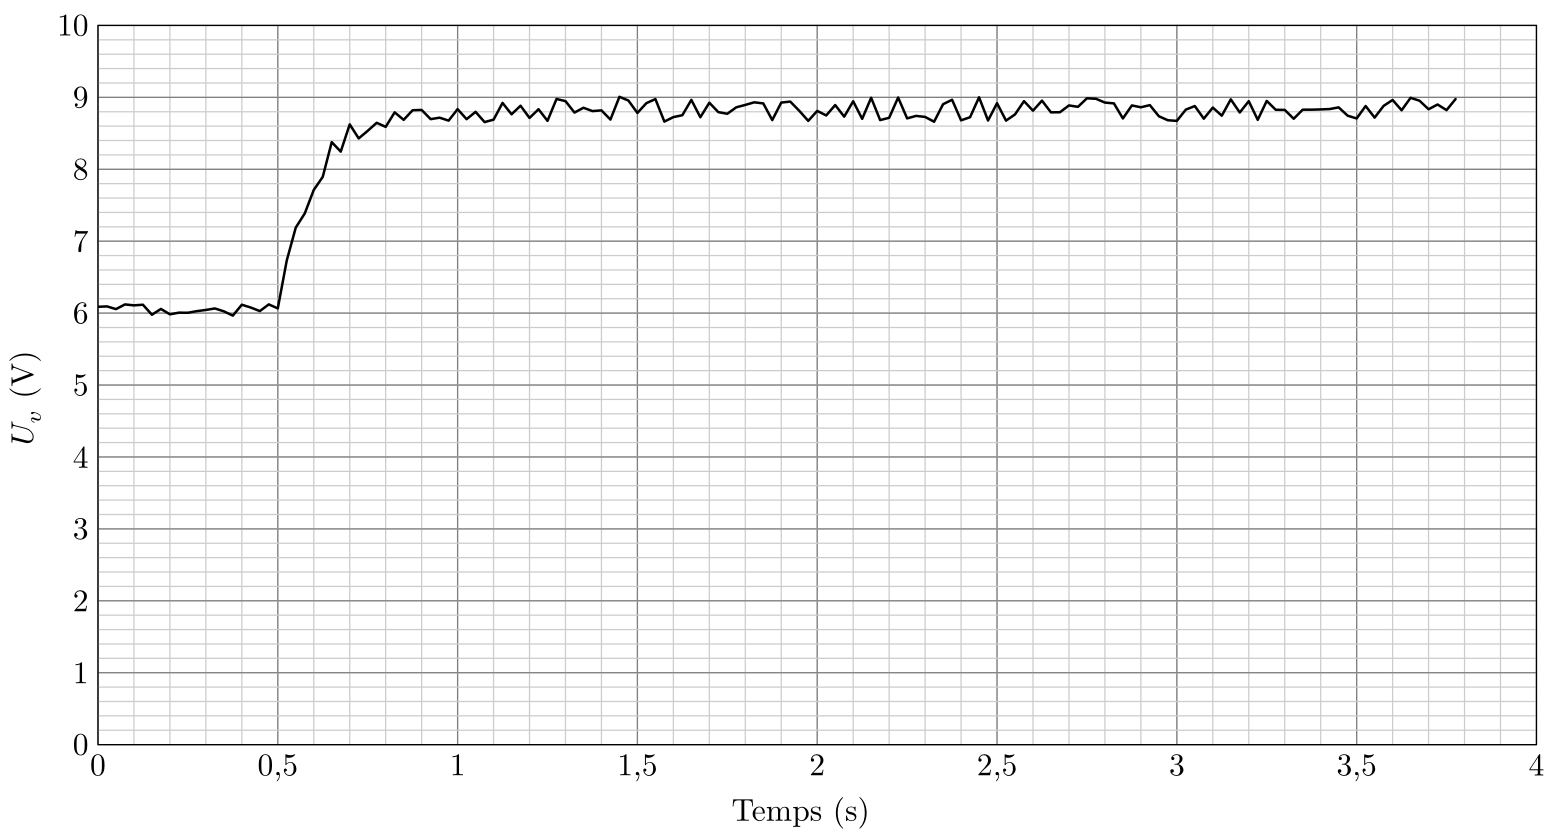
\includegraphics[width=0.8\linewidth]{img/DR04}
\end{center}}{\begin{center}
  \def\svgwidth{.5\textwidth}
  \input{img/DR04_cor.pdf_tex}
\end{center}

On reconnaît un ordre 1 avec un gain $K=\frac{U_v(+\infty)-U(0)}{\Delta \alpha}=\dfrac{8.8-6}{50}=\dfrac{2.8}{50}=5.6\cdot 10^{-2}V\cdot inc^{-1}$ et une constante de temps $\tau=0.15s$.

$\frac{U_v(p)}{\alpha(p)}=\frac{\omega_m(p)\cdot K_{gen}}{\alpha(p)}=K_{gen}\cdot H_v(p)$, donc $H_v(p)=\frac{k}{K_{gen}}\cdot \frac{1}{1+\tau\cdot p}=\frac{0.46}{1+0.1\cdot p}$ 

}

\reponse{3}{}{$H_{BO}(p)=K_c\cdot K_v\cdot \dfrac{K_m}{1+\tau\cdot p}\cdot\frac{K_{red}}{p}\cdot K_{pot}\cdot K_{CAN}$

$H_{BO}(p)$ est de classe 1 donc l'erreur statique est nulle (en absence de perturbation au niveau du moteur qui serait avant l'intégration). L'asservissement permet de suivre parfaitement la consigne de position.}

\ifdef{\public}{\newpage}

\reponse{4}{\begin{center}
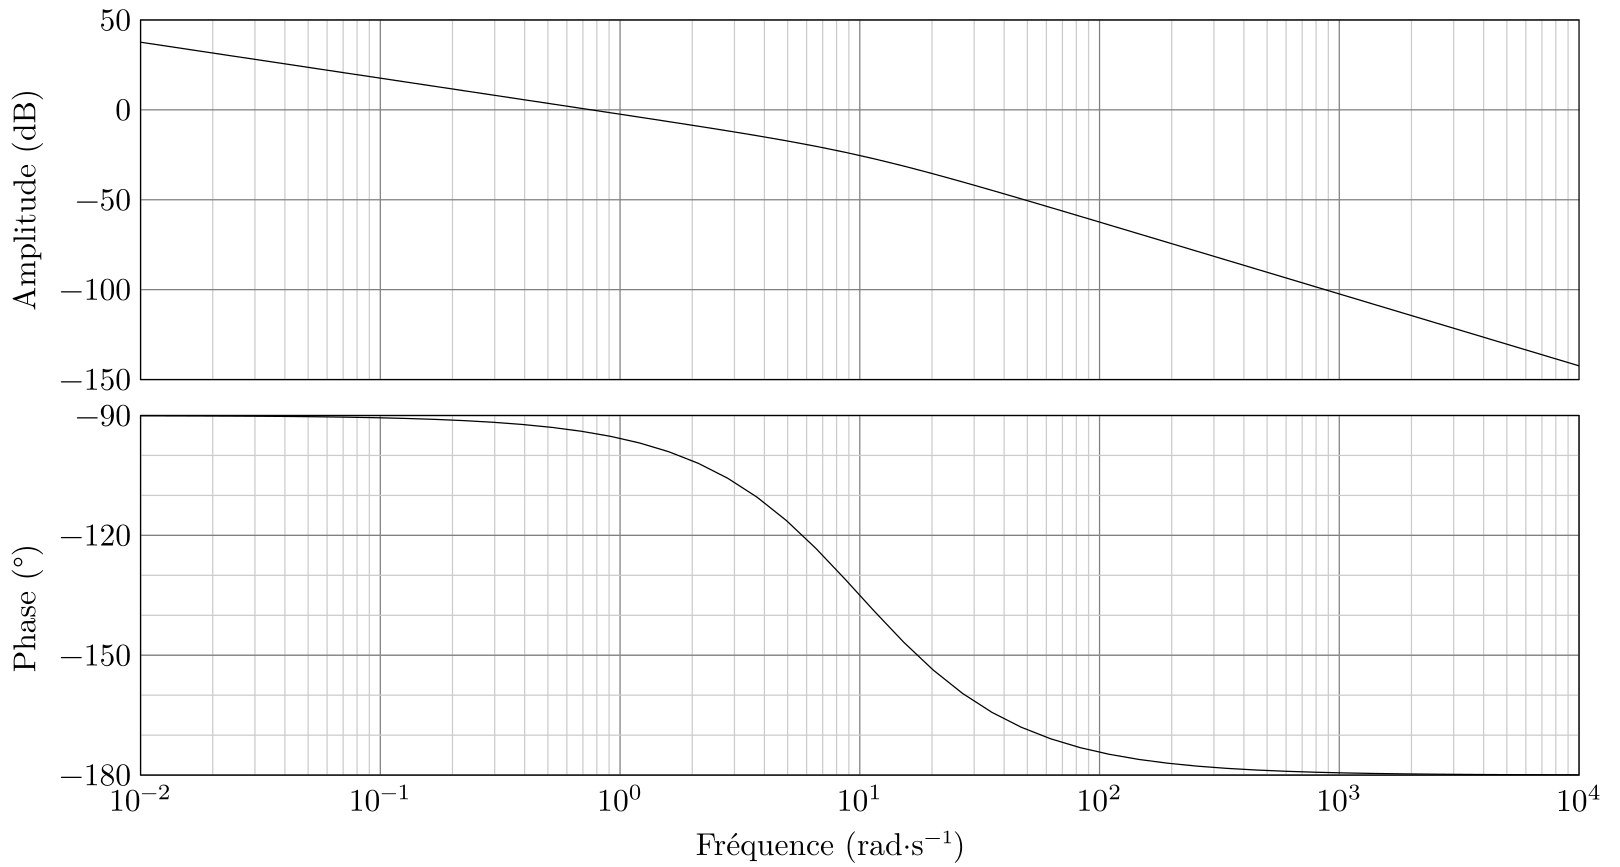
\includegraphics[width=0.8\linewidth]{img/DR05}
\end{center}}{\begin{center}
  \def\svgwidth{.9\textwidth}
  \input{img/DR05_cor.pdf_tex}
\end{center}

C'est un système d'ordre 2 et de classe 1.

Son fonction de transfert est $H(p)=\dfrac{K}{p`cdot (1+\tau\cdot p}$.

Avec $\tau=0.1$ et $K\approx 1$
}

\reponse{6}{}{$H_{BF}(p)=K_{pot}K_{CAN}K_cK_v\dfrac{K_m}{1+\tau\cdot p}\cdot\dfrac{K_{red}}{p}\cdot\dfrac{1}{1+K_{pot}K_{CAN}K_cK_v\dfrac{K_m}{1+\tau\cdot p}\cdot\dfrac{K_{red}}{p}}$

$H_{BF}(p)=\dfrac{1}{1+\dfrac{1}{K_{pot}K_{CAN}K_cK_vK_mK_{red}}\cdot p+\dfrac{\tau}{K_{pot}K_{CAN}K_cK_vK_mK_{red}}\cdot p^2}$

En prenant la forme du second ordre, on obtient:
\begin{itemize}
 \item $K_{BF}=1$,
 \item $\omega_{0BF}=\sqrt{\dfrac{K_{pot}K_{CAN}K_cK_vK_mK_{red}}{\tau}}$,
 \item $\xi_{BF}=\dfrac{1}{2\sqrt{K_{pot}K_{CAN}K_cK_vK_mK_{red}\tau}}$
\end{itemize}}

\ifdef{\public}{\newpage}

\reponse{4}{}{Le dépassement est inférieur à 5\% si $\xi\geq \dfrac{\sqrt{2}}{2}$.

Donc, $K_c\leq \dfrac{1}{2K_{pot}K_{CAN}K_vK_mK_{red}\tau}=\dfrac{1}{2K_{BO}\tau}$

Donc, $K_c\leq\dfrac{1}{2\cot 0,76\cdot 0,1}$

Donc, $K_c\leq\dfrac{10}{1,5}$

Donc, $K_c\leq 6.5$}

\reponse{4}{}{Le temps de réponse le plus court correspond à $\xi=\dfrac{\sqrt{2}}{2}$, dans ce cas, $t_{R5\%}\cdot \omega_0=3$, donc $\left(\omega_0=\sqrt{\dfrac{K_{pot}K_{CAN}K_cK_vK_mK_{red}}{\tau}}\right)\geq\dfrac{3}{t_{R5\%}}$ donc $K_c\geq\dfrac{9}{t_{R5\%}^2}\dfrac{\tau}{K_{pot}K_{CAN}K_cK_vK_mK_{red}}=\dfrac{9}{t_{R5\%}^2}\cdot\dfrac{\tau}{K_{BO}}$

$K_c\geq \dfrac{9}{2^2}\dfrac{0.1}{0.76}$

$K_c\geq \dfrac{0.9}{3}$,

donc $K_c\geq 0,3$.}

\reponse{2}{\begin{center}
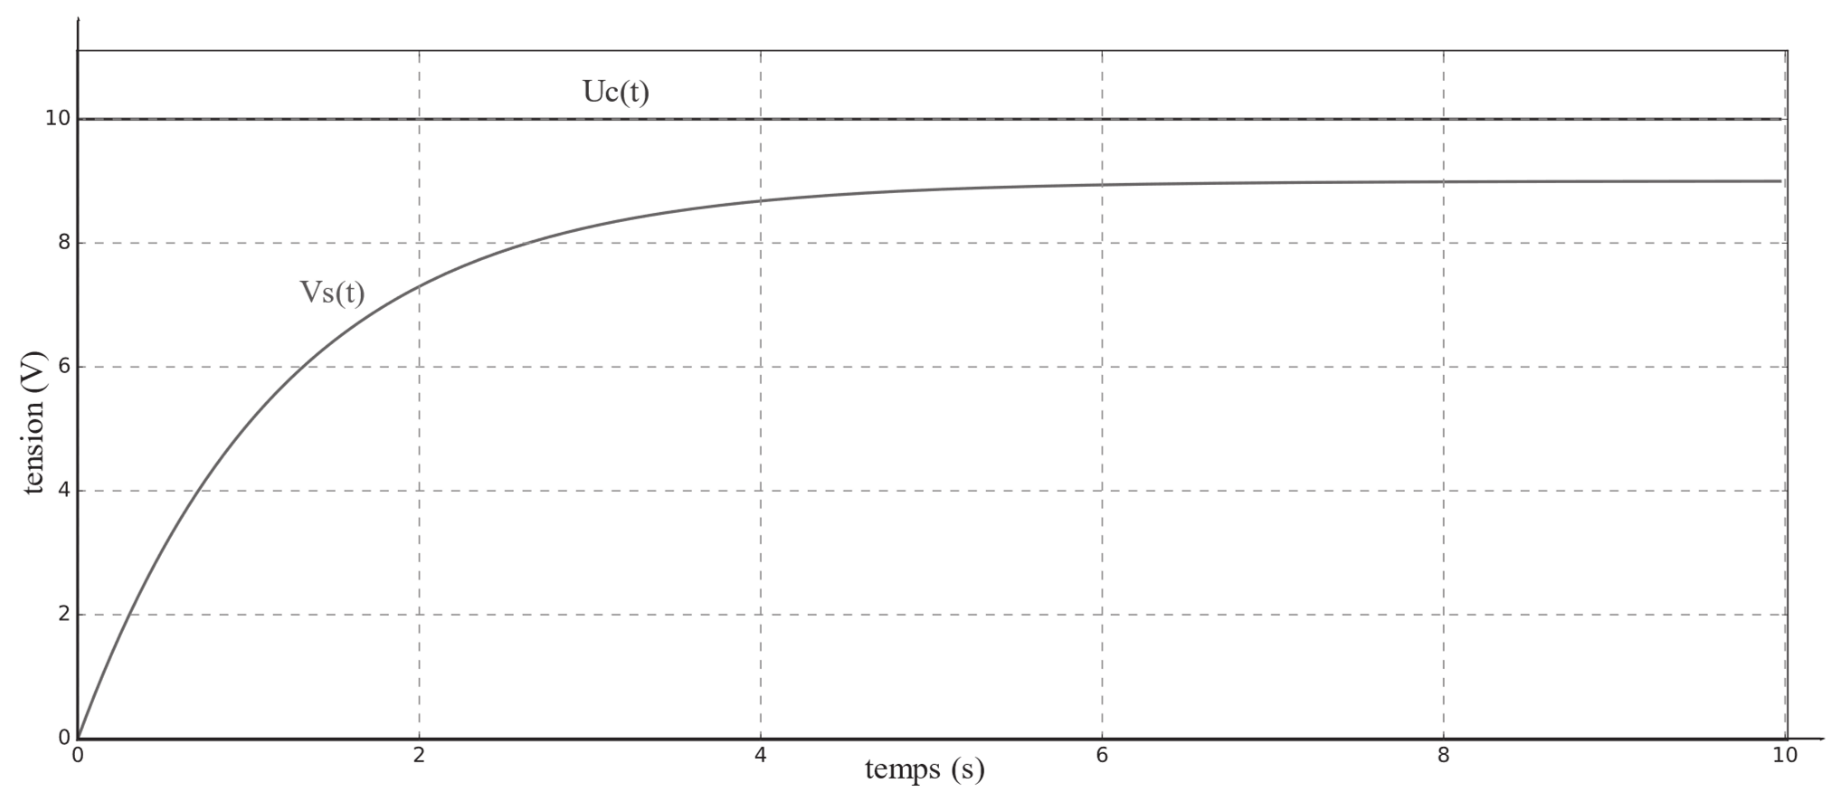
\includegraphics[width=0.7\linewidth]{img/DR06}
\begin{tabular}{|c|c|}
\hline
Critère & Valeurs de $K_c$\\ \hline
Dépassement & \\ \hline
Précision & \\ \hline
Rapidité & \\ \hline
Bilan & \\ \hline
\end{tabular}\end{center}}{
\begin{center}
  \def\svgwidth{.9\textwidth}
  \input{img/DR06_cor.pdf_tex}
\begin{tabular}{|c|c|}
\hline
Critère & Valeurs de $K_c$\\ \hline
Dépassement & $K_c\leq 6.5$\\ \hline
Précision & $K_c$ indifférent\\ \hline
Rapidité & $0.3\leq K_c$\\ \hline
Bilan & $0.3\leq K_c\leq 6.5$\\ \hline
\end{tabular}\end{center}}

\ifdef{\public}{\newpage}


\reponse{5}{}{\begin{center}
  \def\svgwidth{.5\textwidth}
  \input{img/graphe_liaisons.pdf_tex}
  \end{center}}
  

\reponse{7}{}{
\begin{itemize}
 \item Sphère-plan D : $\overrightarrow{M_{D,O_D\rightarrow 1}}=\vec{0}$,
 \item Sphère-plan E : $\overrightarrow{M_{D,O_E\rightarrow 1}}=2d\cdot N_E\vec{x}$,
 \item Poids du cycliste : $\overrightarrow{M_{D,p\rightarrow c}}=-(d-c)mg\vec{x}$,
 \item Poids du vélo : $\overrightarrow{M_{D,p\rightarrow 1}}=-dm_1g\vec{x}$.
\end{itemize}

$\overrightarrow{\delta_{D,c/0}}=\overrightarrow{M_{D,O_D\rightarrow 1}}+\overrightarrow{M_{D,O_E\rightarrow 1}}+\overrightarrow{M_{D,p\rightarrow c}}+\overrightarrow{M_{D,p\rightarrow 1}}$

En projection sur $\vec{x}$ : $(b+e)\cdot m\cdot\gamma=0+2dN_E-(d-c)mg-dm_1g$

Soit $N_E=\dfrac{m\cdot\gamma\cdot (b+e)+(dm_1+(d-c)m)\cdot g}{2d}$}

\reponse{5}{}{
A la limite du basculement $N_E=0$ donc $m\gamma(b+e)+(dm_1+(d-c)m)g=0$

$\gamma=-\dfrac{dm_1+(d-c)m}{(b+e)m}g=-\dfrac{0.25\times 56 +(0.25-0.2)\times 125}{(1.1+0.05)\cdot 56}9.81=-\dfrac{14+6.5}{60}\cdot 10\approx -\dfrac{20}{60}\cdot 10$

$\gamma\approx -3m\cdot s^{-1}$

Le cahier des charges est respecté car le vélo restera stable sous une accélération de $0.5m\cdot s^{-2} < |\gamma| = 3.08m\cdot s^{-1}$.}

\ifdef{\public}{\newpage}

\reponse{5}{}{$\overrightarrow{V_{B\in 1/0}}=\overrightarrow{V_{A\in 1/0}}+\overrightarrow{BA}\wedge\overrightarrow{\Omega_{1/0}}=\vec{0}-R\cdot\vec{y}_1\wedge\dot{\theta}_1\vec{z}_1$

$\overrightarrow{V_{B\in 1/0}}=-R\cdot\dot{\theta}_1\cdot\vec{x}_1$

$\overrightarrow{V_{B\in 2/0}}=\dot{\lambda}(t)\cdot\vec{x}_2+\lambda(t)\left[\dfrac{\vec{x}_2}{dt}\right]_{R_0}$

$\overrightarrow{V_{B\in 2/0}}=\dot{\lambda}(t)\cdot\vec{x}_2+\lambda(t)\cdot \dot{\theta}_2\cdot\vec{y}_2$
}

\reponse{4}{}{
$\overrightarrow{V_{B\in 2/0}}=\overrightarrow{V_{B\in 1/0}}$ car liaison pivot entre 1 et 2 en B.

Projeter sur $\vec{x}_2$: $-R\cdot \dot{\theta}_1\cdot\vec{x}_1\cdot\vec{x}_2=\dot{\lambda}(t)$

Soit $\dot{\lambda}(t) = -R\cdot\dot{\theta}_1\cdot cos(\theta_2-\theta_1)$.
}

\reponse{4}{}{$\dot{\lambda}_{max}=-R\cdot \dot{\theta}_1\cdot cos(\theta_2-\theta_1)_{max}$

$\dot{\lambda}_{max}=-0.25\cdot 0.023\cdot 0.9=-10^{-3}\cdot\dfrac{23}{4}\cdot 0.9$

$\dot{\lambda}_{max}=-10^{-3}\cdot(5.75-0.575)=-5.18\cdot 10^{-3}\cdot s^{-1}$
}

\reponse{5}{}{
\begin{itemize}
 \item Puissance utile : $P_u=F\cdot \dot{\lambda}_{max}$,
 \item Puissance électrique à fournir au moteur : $P=\dfrac{P_u}{\eta_v}=\dfrac{F\cdot \dot{\lambda}_{max}}{\eta_v}=\dfrac{1500\cdot5.2 \cdot 10^{-3}}{0.3}=14.4W$,
 \item Puissance absorbée maximale : $P_{a,max}=U\cdot I_{max}\cdot cos\phi=120\cdot 0.5\cdot 0.8=48W$
\end{itemize}

$P_{a,max}=48W>P=14,4W$ donc la puissance disponible sera suffisante pour incliner le vélo.}

\reponse{0}{\begin{tabular}{|m{4cm}|m{2.5cm}|m{9cm}|}
\hline
Exigence & Validation & Démarche \\ \hline
id 1.2.1 : Permettre un parcours virtuel &  &  \\
&  &  \\
&  &  \\
&  &  \\
&  &  \\
&  &  \\
\hline
id 1.2.2 : Donner la sensation de résistance au pédalage &   & \\
&  &  \\
&  &  \\
&  &  \\
&  &  \\
&  &  \\
\hline
id 1.1 : Incliner le vélo autour de l'axe longitudinal &   &  \\
&  &  \\
&  &  \\
&  &  \\
&  &  \\
&  &  \\
\hline
\end{tabular}}{
\begin{tabular}{|m{4cm}|m{2.5cm}|m{9cm}|}
\hline
Exigence & Validation & Démarche \\ \hline
id 1.2.1 : Permettre un parcours virtuel & validé &  paramétrage de la connexion réseau, expérimentation : mesure de la puissance et de la bande
passante du signal WIFI reçu par le vélo \\ \hline
id 1.2.2 : Donner la sensation de résistance au pédalage & validé & modèle de l'action résistive jusqu'à 4° + programmation
de la loi de commande
modèle de l'asservissement pour régler le correcteur
simulation pour vérifier les performances
\\ \hline
id 1.1 : Incliner le vélo autour de l'axe longitudinal & validé & 
modèle cinématique pour établir la vitesse maximale du
vérin à prévoir modèle énergétique pour vérifier le dimensionnement
de l'alimentation. \\ \hline
\end{tabular}}

\reponse{0}{
\begin{tabular}{|m{3.5cm}|m{6cm}|m{6cm}|}
\hline
& Inconvénients & Avantages \\ \hline
Vélo Pro-Form TDF & & \\
&  &  \\
&  &  \\
&  &  \\
&  &  \\
&  &  \\
\hline
Vélo traditionnel & & \\
&  &  \\
&  &  \\
&  &  \\
&  &  \\
&  &  \\
\hline
\end{tabular}}{
\begin{tabular}{|m{3.5cm}|m{6cm}|m{6cm}|}
\hline
& Inconvénients & Avantages \\ \hline
Vélo Pro-Form TDF & Nécessité du Wifi et d'internet
Consomme de l'énergie
Le contrôle de l'effort dépend du parcours
Plus cher et sans doute plus lourd
Risque de pannes important
& Plus ludique : immersion
Plus stimulant : le parcours
éventuellement trop difficile est
un challenge
\\ \hline
Vélo traditionnel & Nécessité de régler l'effort manuellement
Moins stimulant : pas d'immersion, challenge moins concret (passage d'un
niveau d'effort au suivant)
& 
Effort toujours adapté à l'intensité souhaitée,
Moins cher et sans doute plus facile à déplacer,
Pas besoin de se connecter
\\ \hline
\end{tabular}}

\end{document}
